\documentclass[11pt]{article}

\usepackage[utf8]{inputenc}
\usepackage[T1]{fontenc}
\usepackage[a4paper,margin=0.85in]{geometry}
\usepackage{graphicx}
\usepackage{subcaption}
\usepackage{float}
\usepackage{booktabs}
\usepackage{array}
\usepackage{enumitem}
\usepackage{microtype}
\usepackage[hidelinks]{hyperref}
\usepackage{xcolor}
\usepackage{listings}
\usepackage{amsmath}
\setlist{nosep,leftmargin=*}
\setlength{\parindent}{0pt}
\setlength{\parskip}{4pt}
\setcounter{tocdepth}{2}

% ---------- Common commands ----------
\newcommand{\evidencebox}[1]{%
  \fbox{\parbox[c][4cm][c]{0.92\linewidth}{\centering
  \textbf{IMAGE / EVIDENCE PLACEHOLDER}\\[3pt]#1}}%
}

\newcommand{\smallevidencebox}[1]{%
  \fbox{\parbox[c][3cm][c]{0.90\linewidth}{\centering
  \small\textbf{IMAGE / EVIDENCE PLACEHOLDER}\\[2pt]#1}}%
}

\newcommand{\TODO}[1]{\textcolor{red}{[TODO: #1]}}

% ---------- Team ----------
\newcommand{\StudentOne}{Abhi Jain (23B0903)}
\newcommand{\StudentTwo}{Deshank Pratap Singh (23B0938)}
\newcommand{\StudentThree}{Dhruv Jain (23B0942)}
\newcommand{\StudentFour}{Sameer Arvind Patil (23B1035)}

\begin{document}

% ============================================================
% TITLE
% ============================================================

\begin{titlepage}
    \centering
    {\scshape\bfseries\Huge Advanced Computer Architecture\par}
    \vspace{0.2cm}
    {\scshape\bfseries\Huge (CS-683)\par}
    \vspace{0.8cm}
    {\huge \textbf{Programming Assignment 1 \\ Task 2: Matrix Multiplication for Inference}\par
    }
    \vspace{1cm}

    {\Large \StudentOne\par}
    {\Large \StudentTwo\par}
    {\Large \StudentThree\par}
    {\Large \StudentFour\par}
    \vspace{0.5cm}
    
    \vfill
    {\large Autumn 2026\par}
  \end{titlepage}
  
\tableofcontents

\newpage
% \section{Task 2: Matrix Multiplication for Inference}
% ============================================================
% 2A
% ============================================================
\section{Task 2A: Software Prefetching}

\subsection{Experimental Setup}
\begin{itemize}
    \item CPU: Intel x86 architecture (Tested on HP Pavilion Laptop)
    \item Matrix dimensions: $128 \times 128$ to $2048 \times 2048$
    \item Prefetch distances: Swept across multiple values; 32 floats (2 cache lines) identified as optimal
    \item Cache fill levels: T0, T1, T2, NTA
    \item Performance counters: \texttt{instructions}, \texttt{cpu\_core/L1D.REPLACEMENT/}, \texttt{l2\_rqsts.miss}, \texttt{LLC-load-misses}, \texttt{sw\_prefetch\_access.any}
    \item Number of runs: 1 warmup, 3 timed repetitions
\end{itemize}

\subsection{Matrix Size Analysis}
As the matrix size increases from $128 \times 128$ up to $2048 \times 2048$, the measured benefit of software prefetching increases in both hardware-prefetcher configurations.

When hardware prefetchers are OFF, the speedup rises from $1.69\times$ at $N=128$ to $2.08\times$ at $N=2048$. With hardware prefetchers ON, the measured gains are similar, from $1.80\times$ to $2.07\times$. In the NT layout, the inner $K$ accesses are contiguous in both operands, but the kernel still has multiple concurrent streams and repeatedly traverses large rows. These results suggest that explicit prefetching can provide additional benefit even when hardware prefetching is enabled.

\subsection{Execution Time and Speedup}
$$
\text{Speedup} =
\frac{\text{Execution Time without Software Prefetching}}
{\text{Execution Time with Software Prefetching}}
$$

\begin{table}[H]
\centering
\caption{Best Software prefetching configurations (HW Prefetch OFF vs ON)}
\begin{tabular}{l|c|c|c||c|c|c}
\toprule
& \multicolumn{3}{c||}{\textbf{HW Prefetch OFF}} & \multicolumn{3}{c}{\textbf{HW Prefetch ON}} \\
Size & Distance/Hint & Time (ms) & Speedup & Distance/Hint & Time (ms) & Speedup \\
\midrule
$128 \times 128$   & 16 / T1 & 0.4130   & 1.6996$\times$ & 16 / NTA & 0.4116   & 1.8040$\times$ \\
$256 \times 256$   & 16 / T1 & 3.4508   & 1.8003$\times$ & 16 / T1  & 3.4766   & 1.7553$\times$ \\
$512 \times 512$   & 16 / T0 & 28.1323  & 1.8825$\times$ & 64 / T1  & 28.2706  & 1.9187$\times$ \\
$1024 \times 1024$ & 16 / T2 & 227.5796 & 1.9456$\times$ & 256 / T2 & 228.7783 & 2.0067$\times$ \\
$2048 \times 2048$ & 16 / T2 & 1868.4863& 2.0849$\times$ & 64 / T1  & 1864.7300& 2.0702$\times$ \\
\bottomrule
\end{tabular}
\end{table}

\begin{figure}[H]
\centering
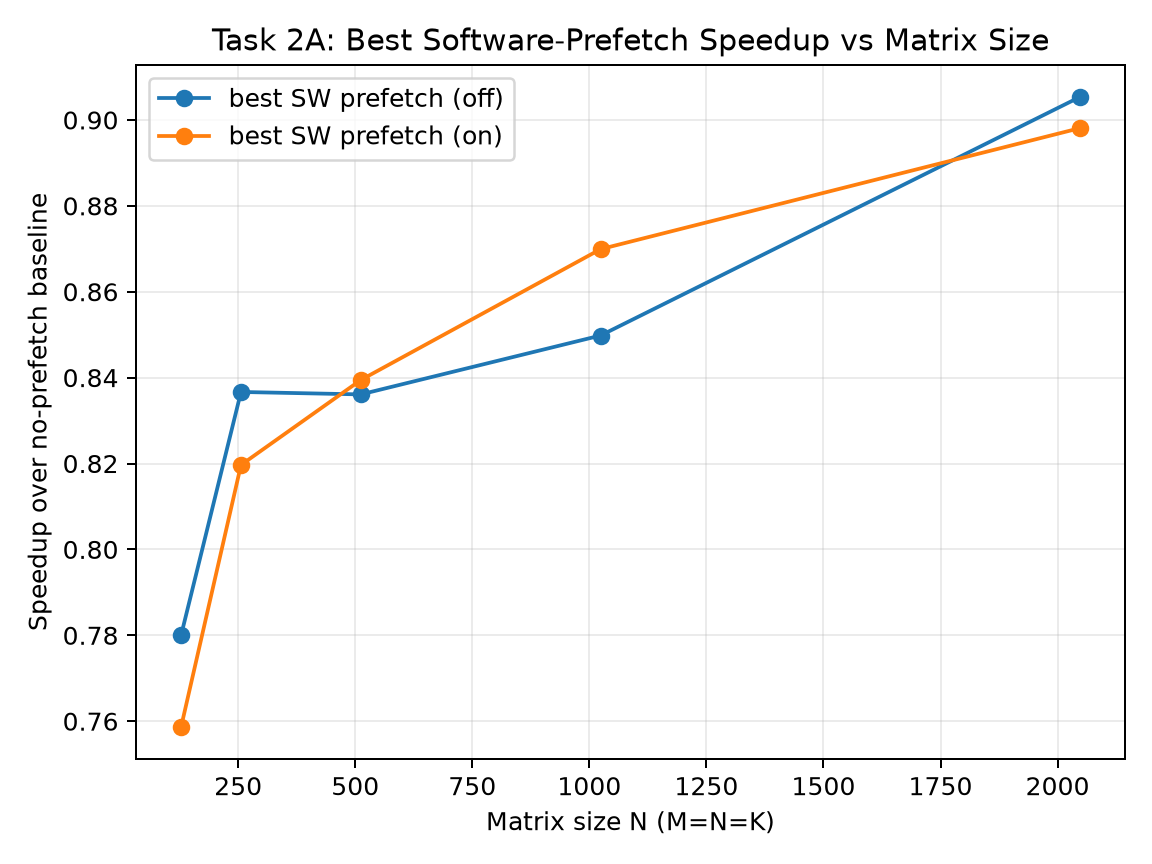
\includegraphics[width=0.75\linewidth]{plots/task2a/task2a_speedup_vs_size.png}
\caption{Software prefetching speedup vs. matrix size (comparing HW prefetcher states).}
\end{figure}

\subsection{CPU Metrics}
\begin{figure}[H]
    \centering
    \begin{subfigure}{0.48\textwidth}
        \centering
        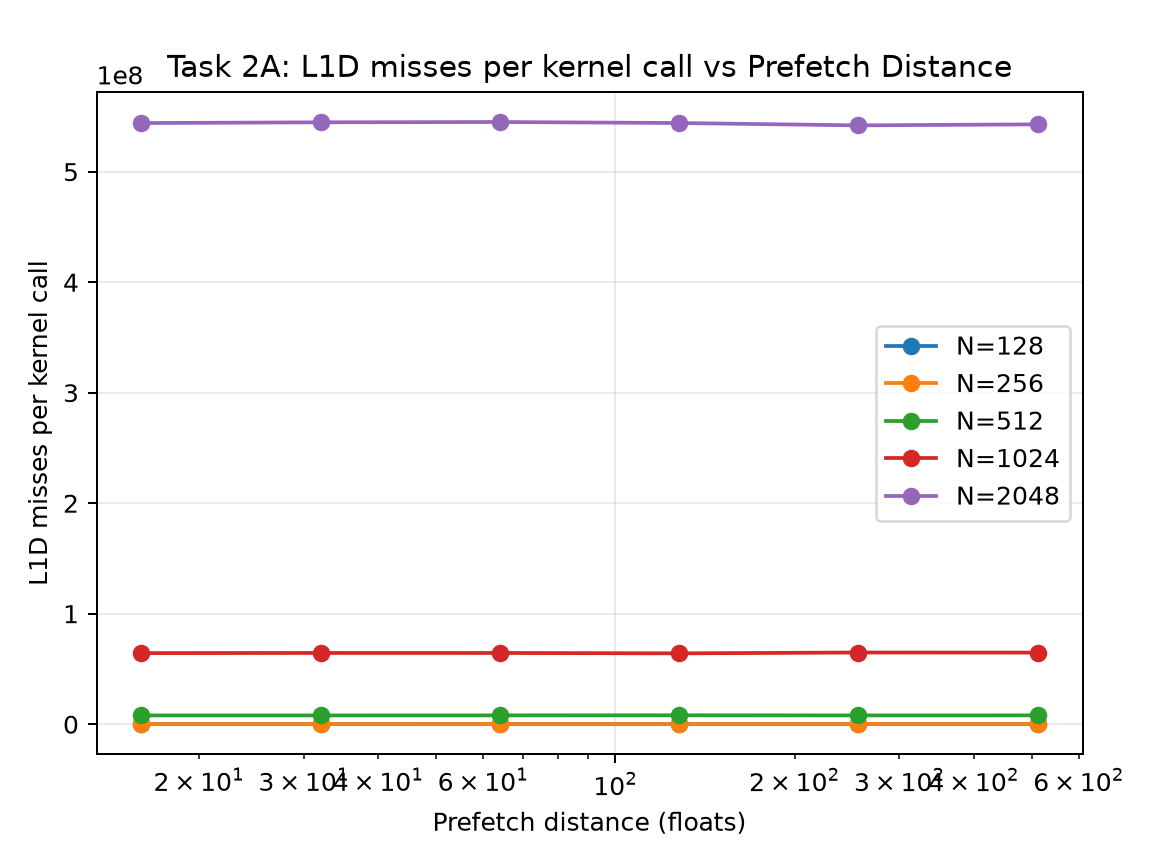
\includegraphics[width=\linewidth]{plots/task2a/task2a_l1d_misses_vs_distance.png}
        \caption{L1D Misses vs Prefetch Distance}
    \end{subfigure}
    \hfill
    \begin{subfigure}{0.48\textwidth}
        \centering
        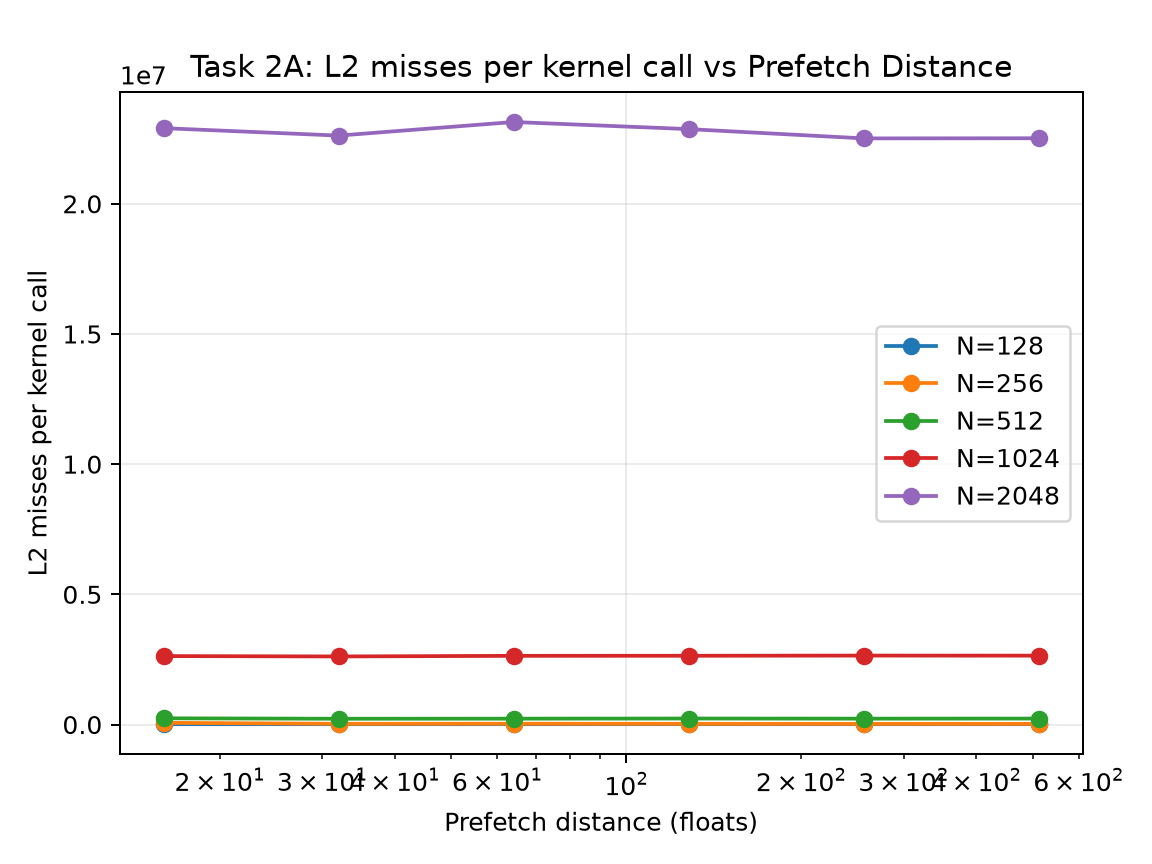
\includegraphics[width=\linewidth]{plots/task2a/task2a_l2_misses_vs_distance.png}
        \caption{L2 Misses vs Prefetch Distance}
    \end{subfigure}
    \vspace{1em}
    \begin{subfigure}{0.48\textwidth}
        \centering
        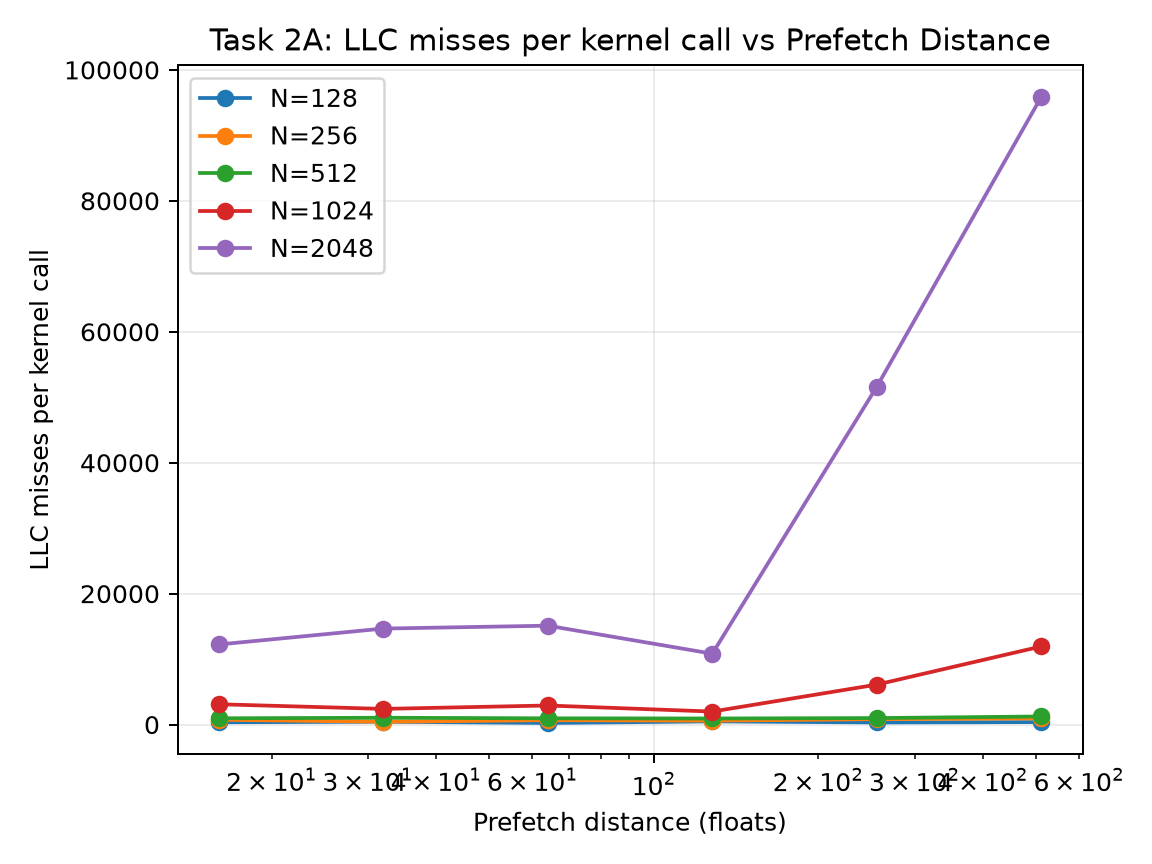
\includegraphics[width=\linewidth]{plots/task2a/task2a_llc_misses_vs_distance.png}
        \caption{LLC Misses vs Prefetch Distance}
    \end{subfigure}
    \hfill
    \begin{subfigure}{0.48\textwidth}
        \centering
        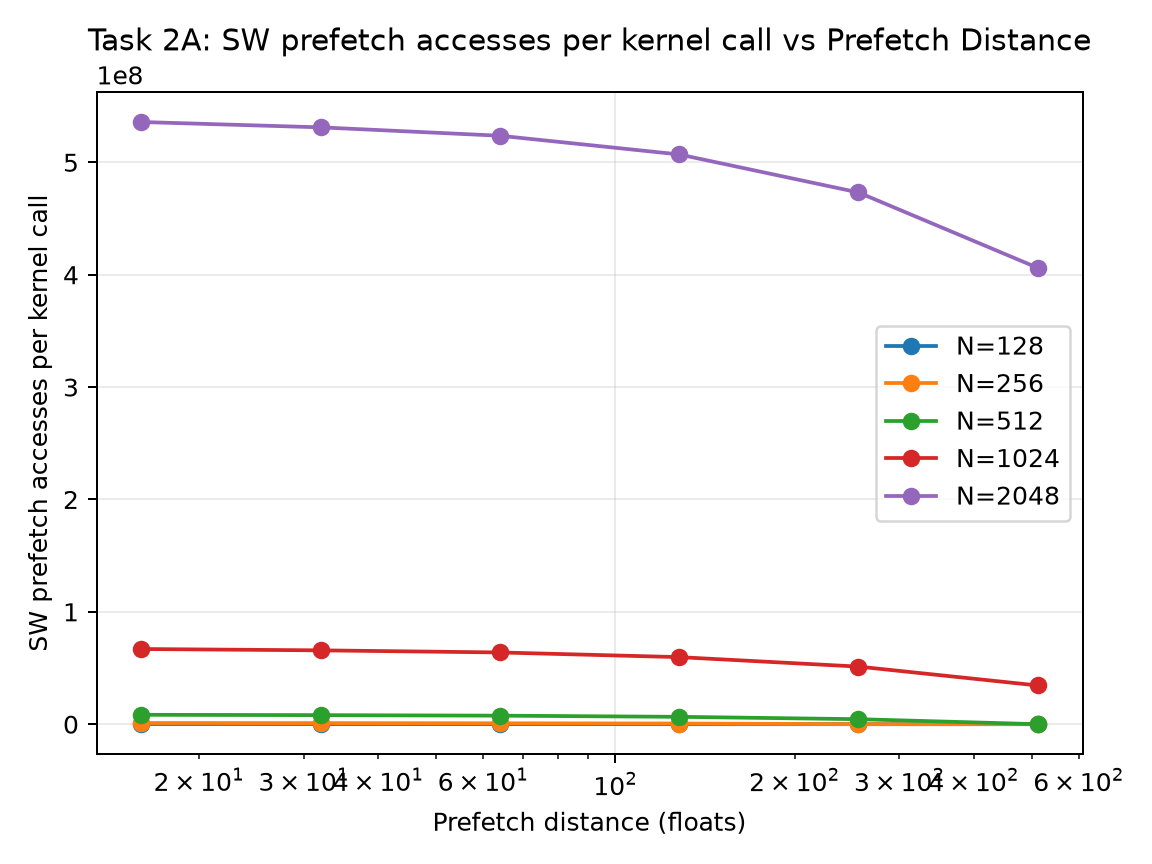
\includegraphics[width=\linewidth]{plots/task2a/task2a_sw_prefetch_access_vs_distance.png}
        \caption{SW Prefetch Accesses vs Distance}
    \end{subfigure}
    \caption{Hardware cache metrics behavior under varying prefetch distances.}
\end{figure}

\subsection{Prefetch Distance}
The prefetch distance determines how far ahead the CPU requests data. Based on the geometric mean across all evaluated sizes, 32 floats (two 64-byte cache lines) gave the best global result. This is distinct from the best configuration at an individual size, which can use another distance. Requests that are too far ahead can add cache pressure or arrive before the data is used.

\begin{figure}[H]
\centering
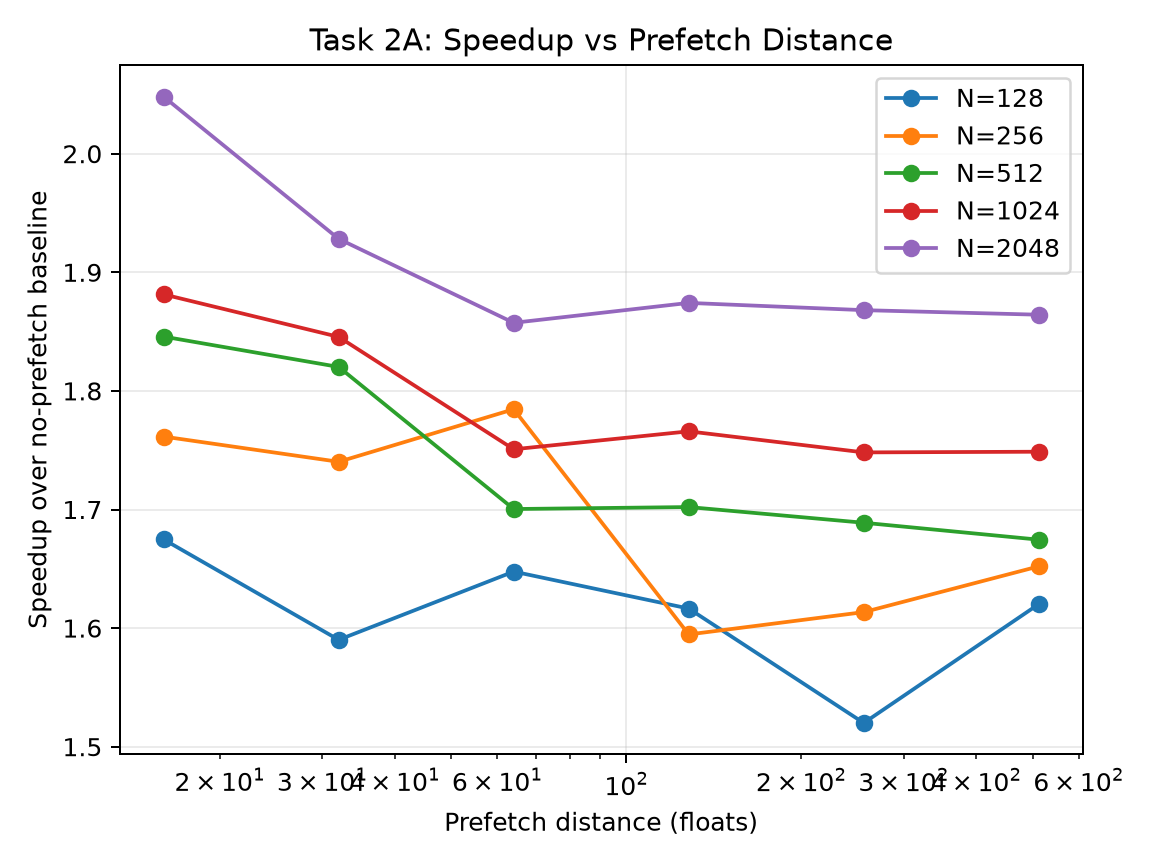
\includegraphics[width=0.75\linewidth]{plots/task2a/task2a_prefetch_distance.png}
\caption{Speedup over baseline across varying prefetch distances.}
\end{figure}

\subsection{Cache Fill Level}
The locality hint expresses the expected temporal reuse of prefetched data; it does not guarantee placement in a particular cache level. Taking the geometric mean across all matrix sizes, \texttt{T1} provided the best overall result. The result is consistent with lower L1 cache pressure than \texttt{T0}, although exact behavior is microarchitecture-dependent.

\begin{figure}[H]
\centering
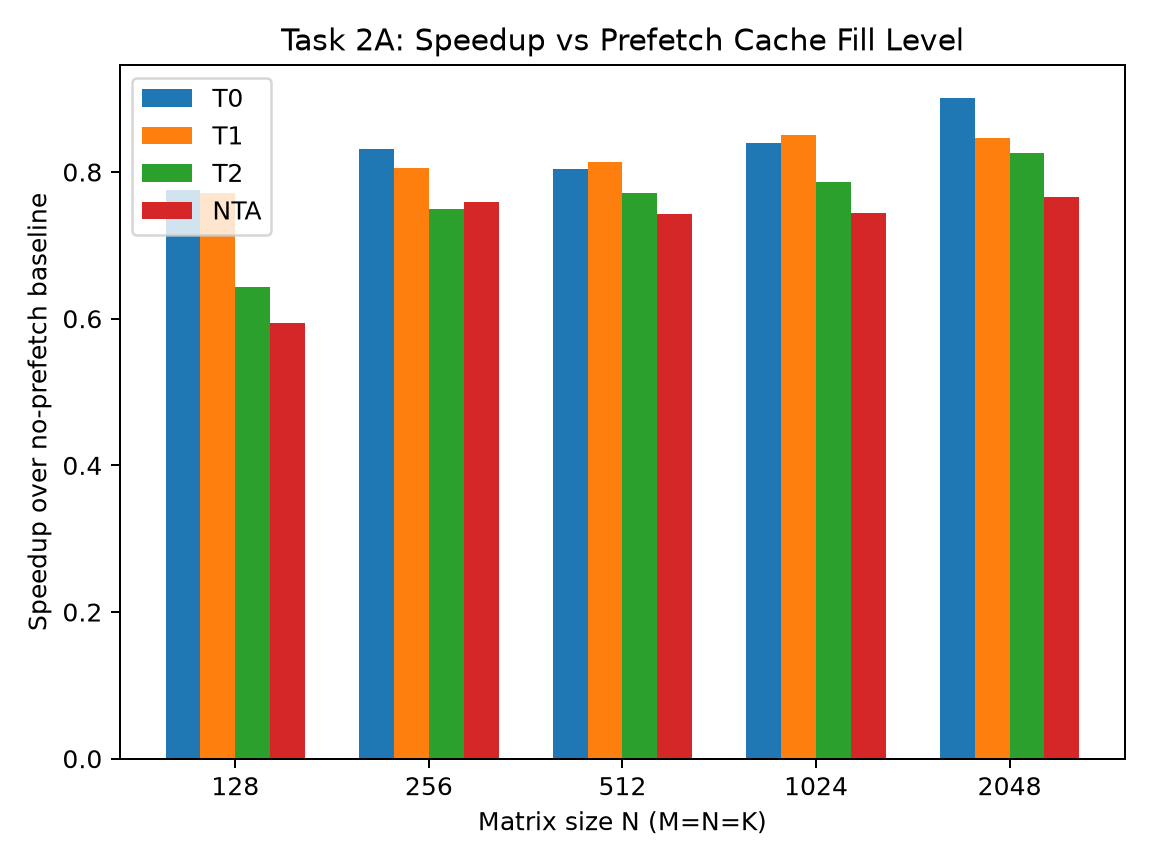
\includegraphics[width=0.75\linewidth]{plots/task2a/task2a_prefetch_level.png}
\caption{Speedup over baseline across varying cache fill levels.}
\end{figure}

\subsection{Hardware Prefetchers}
The results show that software prefetching provided additional benefit with hardware prefetchers enabled. Although the inner $K$ streams are linear, the blocked kernel has several active streams and reuse patterns, so hardware prefetching need not hide every data-delivery delay. The best observed speedup with hardware prefetching enabled was $\sim 2.07\times$.

\begin{figure}[H]
\centering
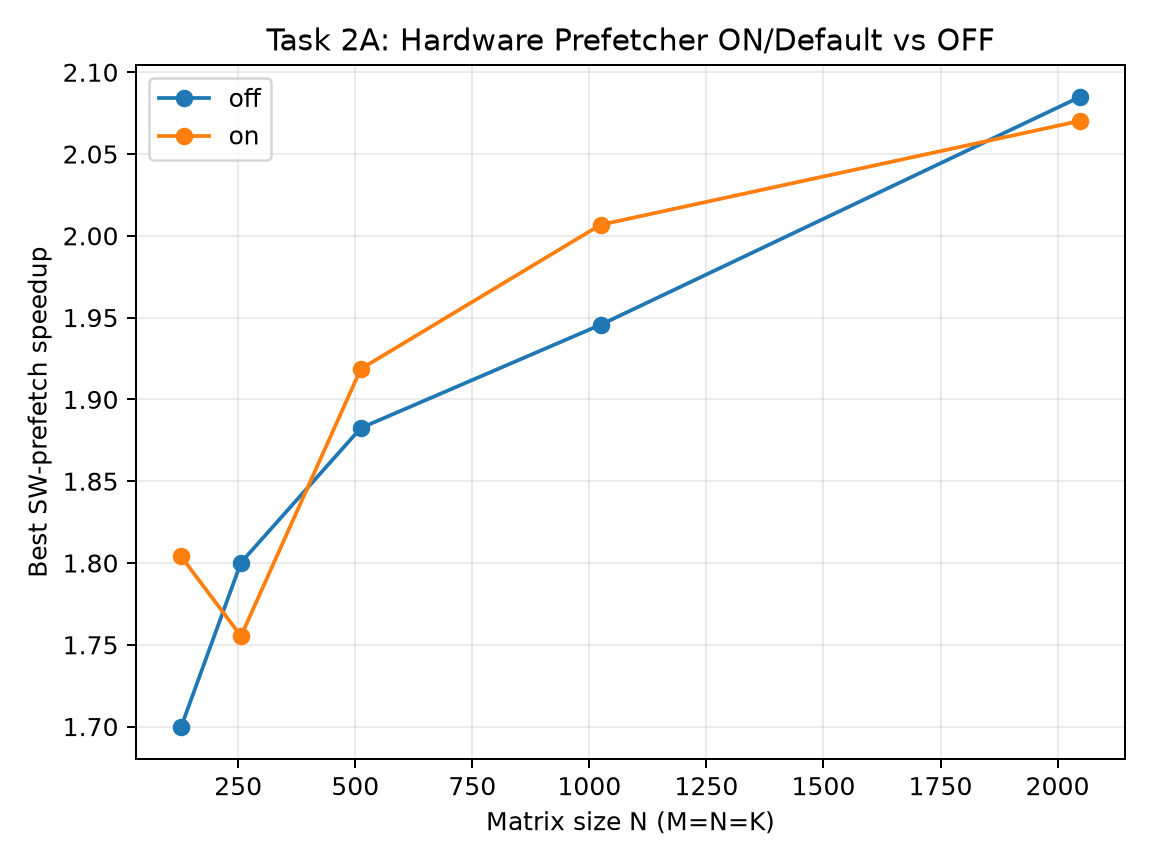
\includegraphics[width=0.75\linewidth]{plots/task2a/task2a_hw_prefetch_on_off.png}
\caption{Hardware prefetcher ON vs OFF comparison.}
\label{fig:hw_prefetch}
\end{figure}

\subsection{Questions}
\begin{enumerate}
    \item \textbf{What trend do you observe in speedup with different matrix sizes?} \\
    In these measurements, speedup increases with matrix size in both hardware-prefetcher configurations, from about $1.7\times$ at $N=128$ to about $2.08\times$ at $N=2048$. This trend is consistent with data-delivery delays becoming a larger fraction of execution time as the working set grows.
    
    \item \textbf{What is the best prefetch distance?} \\
    Based on the geometric mean across all evaluated sizes, 32 floats (which translates to 2 cache lines) is the optimal prefetch distance.
    
    \item \textbf{At what cache fill level do you achieve the maximum speedup?} \\
    The \texttt{T1} hint achieved the maximum geometric-mean speedup. It requests lower temporal locality than \texttt{T0}; the actual cache response is microarchitecture-dependent.
\end{enumerate}

\newpage
% ============================================================
% 2B
% ============================================================

\section{Task 2B: SIMD (Single Instruction Multiple Data)}

\subsection{SIMD Implementation}
To parallelize the SGEMM operation, we implemented a register-blocked SIMD micro-kernel using AVX2 intrinsics. We unrolled the outer loops to compute a $2 \times 4$ block of the output matrix $C$ simultaneously. For the inner dot-product loop across the $K$ dimension, we used \texttt{\_mm256\_loadu\_ps} to fetch 8 elements from both matrices and accumulated the results using \texttt{\_mm256\_fmadd\_ps}. Finally, we implemented a \texttt{horizontal\_sum} helper function using vector extraction and addition to collapse the 8-lane accumulators into scalar values for the final output. 

\subsection{Performance and Instruction Analysis}

As expected, vectorizing the dot product drastically reduced the number of executed instructions. For a $1024 \times 1024$ matrix, the baseline executed $\sim$6.46 billion instructions, whereas the 256-bit SIMD implementation required only $\sim$227 million instructions—a reduction by a factor of roughly $28\times$.

\begin{table}[H]
\centering
\caption{Task 2B Execution Time and Speedup Summary}
\begin{tabular}{lccc}
\toprule
Matrix Size & No SIMD Time (ms) & 128-bit Speedup & 256-bit Speedup \\
\midrule
$128 \times 128$ & 0.76 & 8.67$\times$ & 12.64$\times$ \\
$256 \times 256$ & 6.20 & 9.11$\times$ & 9.87$\times$ \\
$512 \times 512$ & 53.52 & 9.64$\times$ & 12.15$\times$ \\
$1024 \times 1024$ & 446.38 & 9.19$\times$ & 11.49$\times$ \\
$2048 \times 2048$ & 3802.51 & 8.51$\times$ & 10.00$\times$ \\
\bottomrule
\end{tabular}
\end{table}

\begin{figure}[H]
    \centering
    \begin{subfigure}{0.48\textwidth}
        \centering
        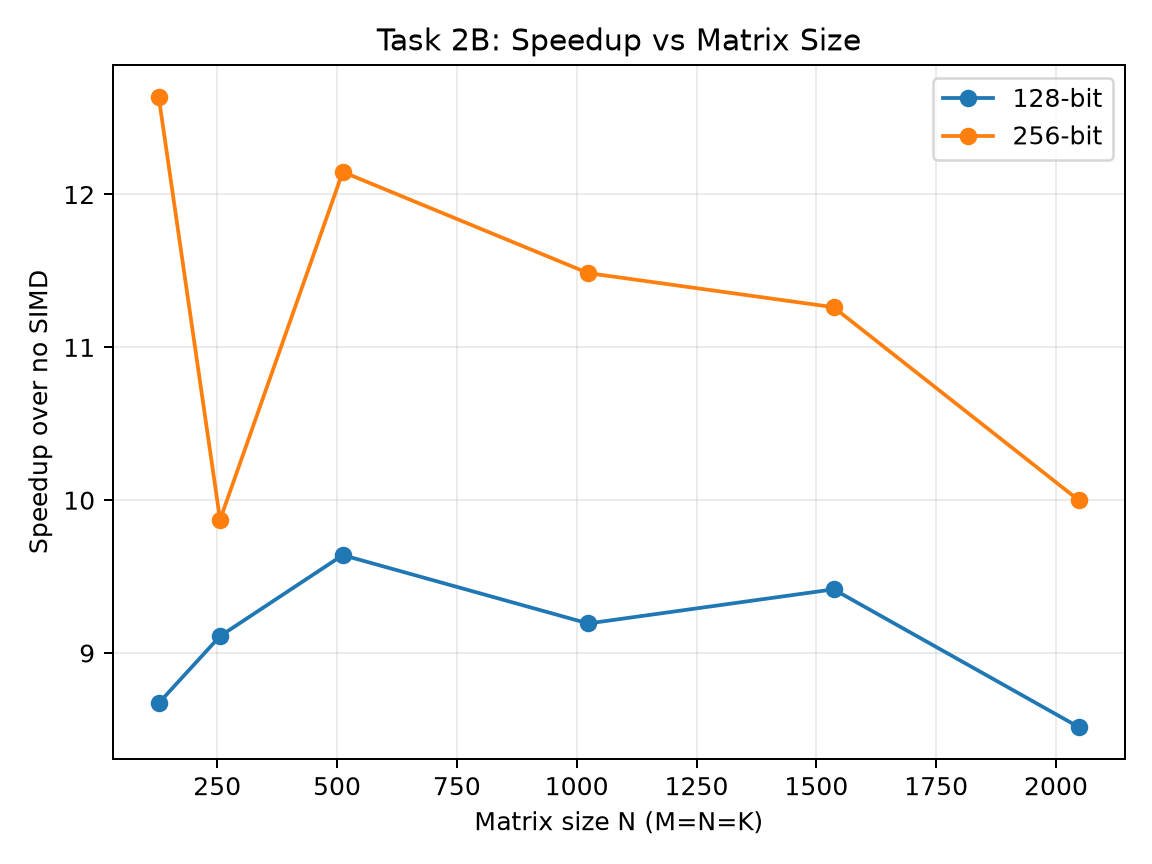
\includegraphics[width=\linewidth]{plots/task2b/task2b_speedup_vs_size.png}
        \caption{Speedup vs Matrix Size}
    \end{subfigure}
    \hfill
    \begin{subfigure}{0.48\textwidth}
        \centering
        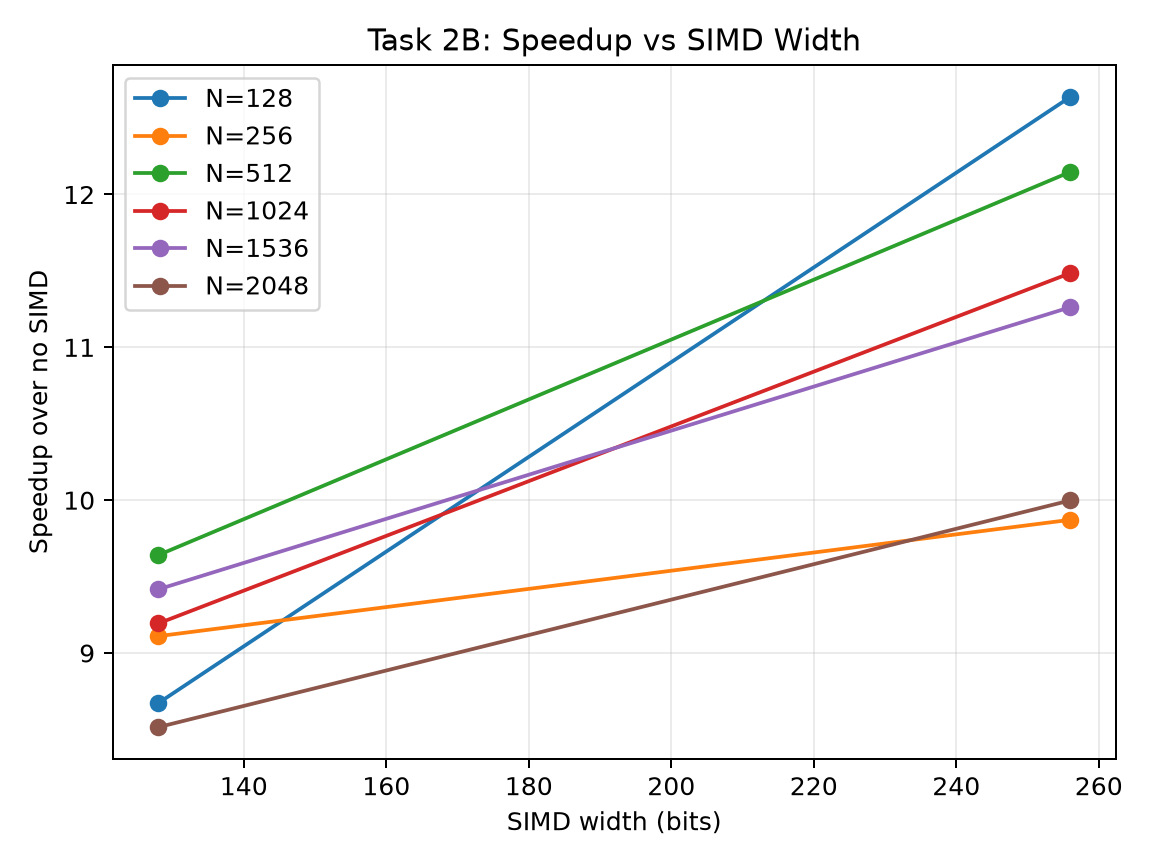
\includegraphics[width=\linewidth]{plots/task2b/task2b_speedup_vs_width.png}
        \caption{Speedup vs SIMD Width}
    \end{subfigure}
    \caption{Performance improvements across varying matrix constraints.}
\end{figure}

\begin{figure}[H]
    \centering
    \begin{subfigure}{0.48\textwidth}
        \centering
        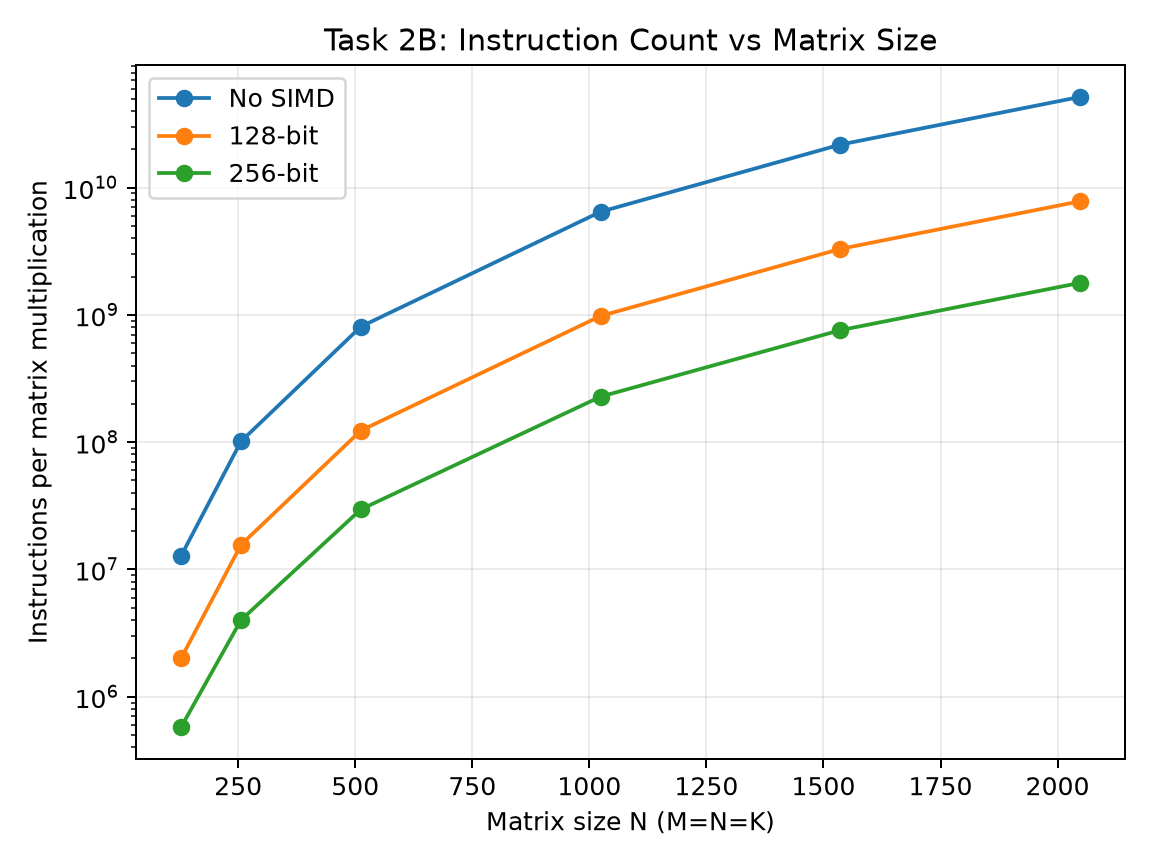
\includegraphics[width=\linewidth]{plots/task2b/task2b_instructions_vs_size.png}
        \caption{Total Instructions vs Size}
    \end{subfigure}
    \hfill
    \begin{subfigure}{0.48\textwidth}
        \centering
        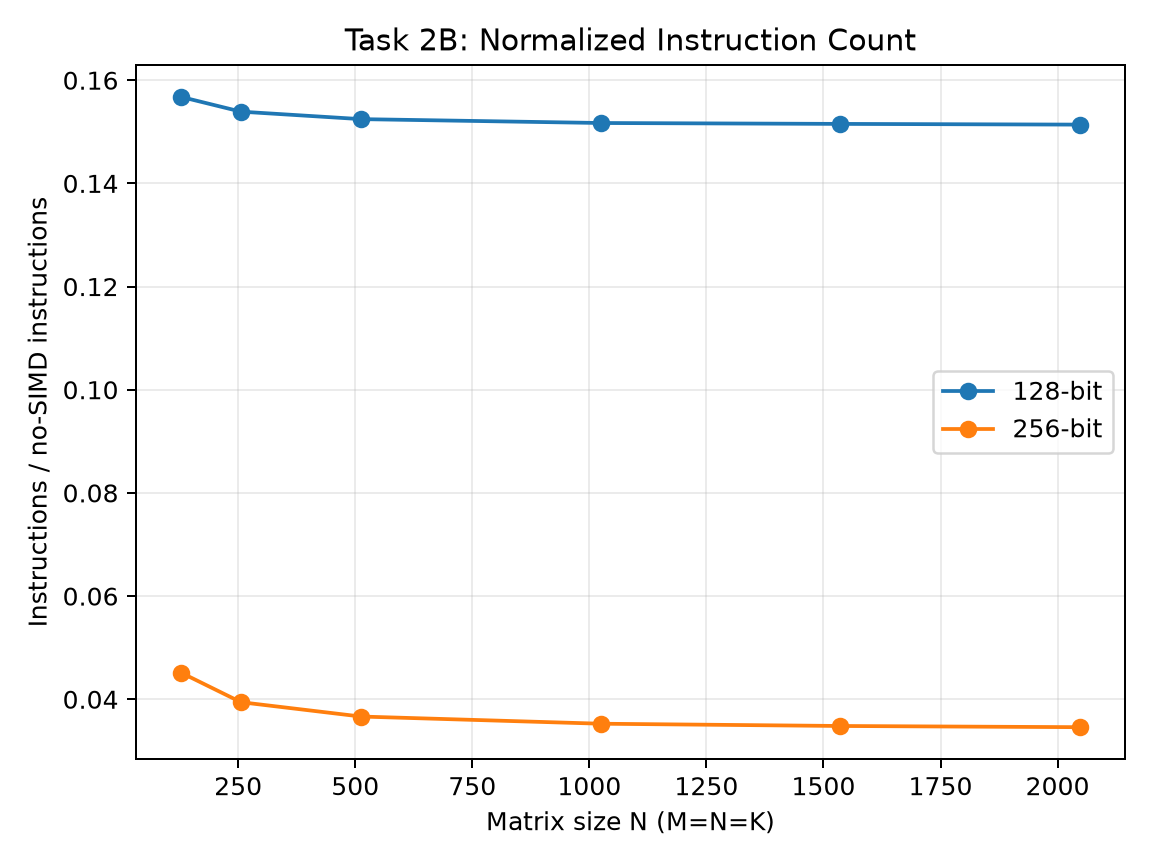
\includegraphics[width=\linewidth]{plots/task2b/task2b_instruction_ratio_vs_size.png}
        \caption{Normalized Instruction Count}
    \end{subfigure}
    \caption{Impact of vectorization on total instruction execution.}
\end{figure}

\begin{figure}[H]
    \centering
    \begin{subfigure}{0.48\textwidth}
        \centering
        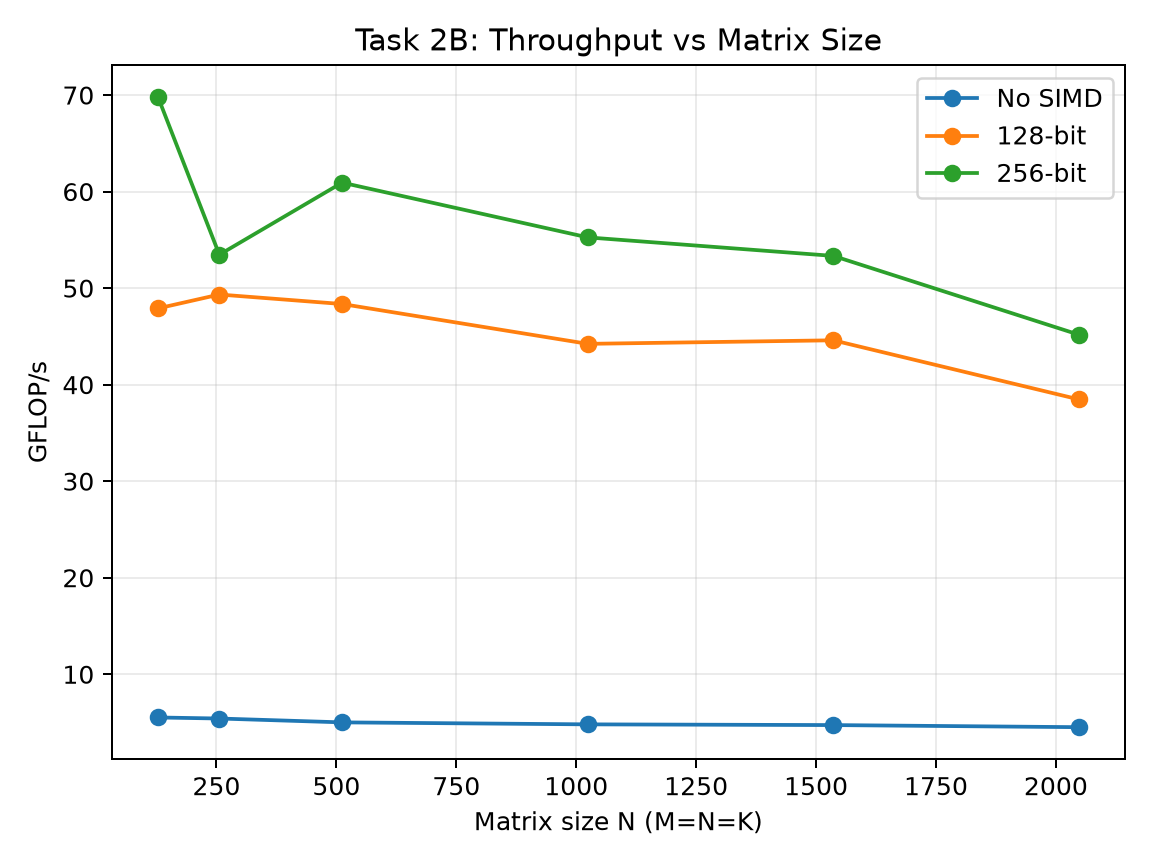
\includegraphics[width=\linewidth]{plots/task2b/task2b_gflops_vs_size.png}
        \caption{Throughput (GFLOP/s) vs Size}
    \end{subfigure}
    \hfill
    \begin{subfigure}{0.48\textwidth}
        \centering
        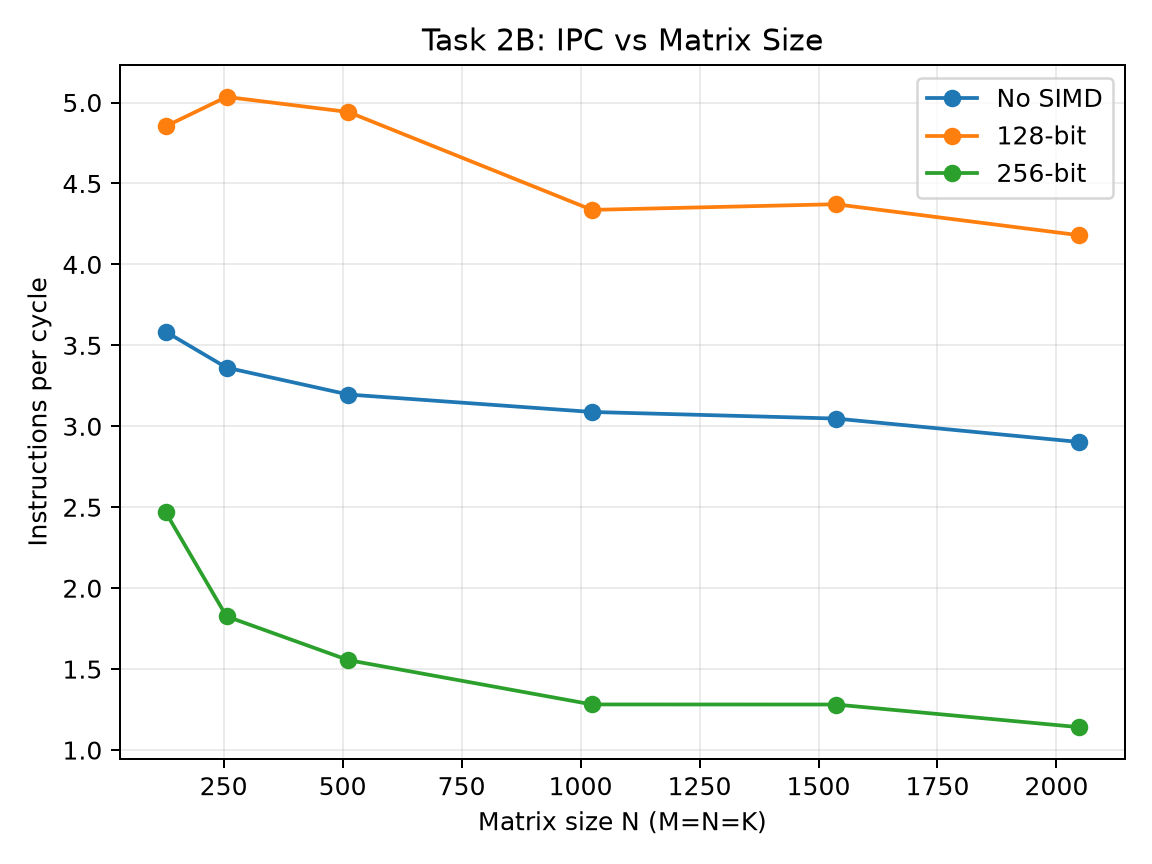
\includegraphics[width=\linewidth]{plots/task2b/task2b_ipc_vs_size.png}
        \caption{IPC vs Size}
    \end{subfigure}
    \caption{Hardware utilization and throughput efficiency.}
\end{figure}


\subsection{Questions}

\begin{enumerate}
    \item \textbf{What trends do you observe in speedup for different combinations of matrix sizes and SIMD widths?} \\
    The 256-bit SIMD implementation strictly outperforms the 128-bit implementation across all matrix sizes. For both widths, the speedup peaks at smaller boundaries (e.g., $12.64\times$ at $N=128$) and gently degrades as the matrix size increases (dropping to $10.00\times$ at $N=2048$). This downward trend indicates that as the matrix footprint grows well beyond the L1/L2 cache capacities, memory bandwidth becomes the primary bottleneck, starving the highly efficient SIMD arithmetic units.
    
    \item \textbf{For which SIMD width do you achieve the maximum speedup?} \\
    We achieved the maximum speedup using the 256-bit SIMD width. It produced a geometric mean speedup of roughly $11.19\times$ across all sizes, compared to the 128-bit version which was consistently slower. This maps directly to the hardware capability: 256-bit registers process 8 single-precision floats per instruction cycle, effectively doubling the raw arithmetic throughput over 128-bit SSE registers.
\end{enumerate}

\newpage
% ============================================================
% 2C
% ============================================================

\section{Task 2C: Software Prefetching + SIMD}

\subsection{Combined Implementation}
In the combined implementation (\texttt{matmul\_optimized.cpp}), the matrix multiplication is first cache-blocked into tiles of $BM=32$ and $BN=32$ to maximize data reuse. Within these tiles, the inner kernel is aggressively unrolled into a $2 \times 4$ micro-kernel utilizing 256-bit AVX2 SIMD intrinsics (\texttt{\_\_m256}). Vectorization is achieved using \texttt{\_mm256\_fmadd\_ps} to perform 8 fused multiply-add operations concurrently. To keep these wide vector units fed, \texttt{\_mm\_prefetch} instructions are interleaved within the innermost $K$-loop, fetching chunks of matrices $A$ and $B$ ahead of the SIMD load instructions. 

\subsection{Experimental Setup}
\begin{itemize}
    \item \textbf{Matrix dimensions:} $128 \times 128$ up to $2048 \times 2048$
    \item \textbf{SIMD Widths:} 128-bit, 256-bit (AVX2)
    \item \textbf{Prefetch distances:} 16, 32, 64, 128, 256, 512 floats
    \item \textbf{Cache fill levels:} T0, T1, T2, NTA
    \item \textbf{Primary Dataset:} Hardware prefetcher enabled (ON)
\end{itemize}

\subsection{Combined Results}

\begin{table}[H]
\centering
\caption{Task 2C combined optimization results (HW Prefetch ON)}
\begin{tabular}{lccccc}
\toprule
Matrix Size & SIMD Width & Prefetch Distance & Level & Time (ms) & Speedup \\
\midrule
$128 \times 128$   & 256 & 512 & T0 & 0.0520  & 15.8273$\times$ \\
$256 \times 256$   & 256 & 16  & T0 & 0.4483  & 17.1198$\times$ \\
$512 \times 512$   & 256 & 32  & T0 & 4.0406  & 14.0673$\times$ \\
$1024 \times 1024$ & 256 & 64  & T0 & 30.9540 & 15.4376$\times$ \\
$2048 \times 2048$ & 256 & 32  & T0 & 289.8732& 14.1236$\times$ \\
\bottomrule
\end{tabular}
\end{table}

\begin{figure}[H]
    \centering
    \begin{subfigure}{0.48\textwidth}
        \centering
        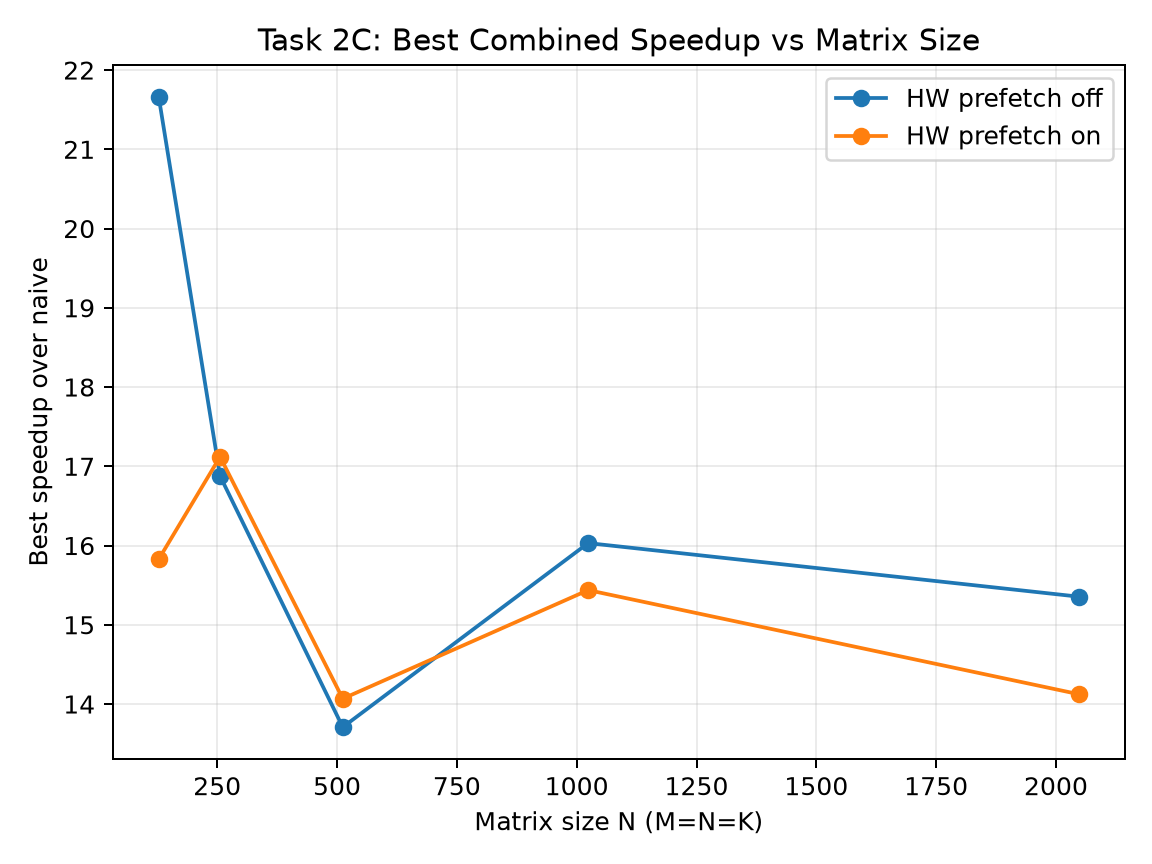
\includegraphics[width=\linewidth]{plots/task2c/task2c_best_speedup_vs_size.png}
        \caption{Combined Speedup vs. Matrix Size}
    \end{subfigure}
    \hfill
    \begin{subfigure}{0.48\textwidth}
        \centering
        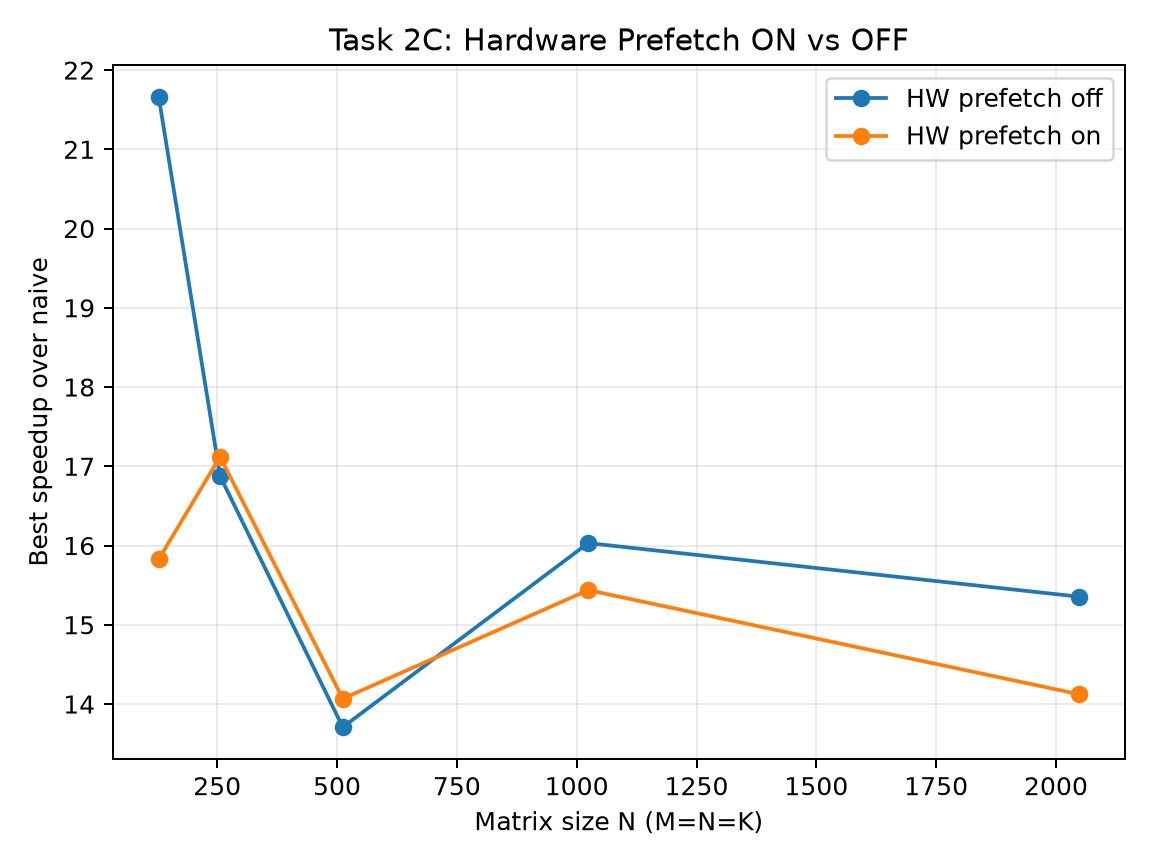
\includegraphics[width=\linewidth]{plots/task2c/task2c_hw_prefetch_on_off.png}
        \caption{Hardware Prefetcher ON vs OFF}
    \end{subfigure}
    \caption{Overall performance scaling of the combined optimizations.}
\end{figure}

\subsection{Analysis}

\subsubsection{SIMD Width and Instruction Count}
Moving from scalar code to 128-bit and then 256-bit SIMD drastically reduces the total number of instructions executed. Because the 256-bit SIMD instructions consume data much faster than scalar code (processing 8 floats per instruction), the CPU pipeline bottleneck shifts away from instruction fetch/decode and lands squarely on memory bandwidth.

\begin{figure}[H]
    \centering
    \begin{subfigure}{0.48\textwidth}
        \centering
        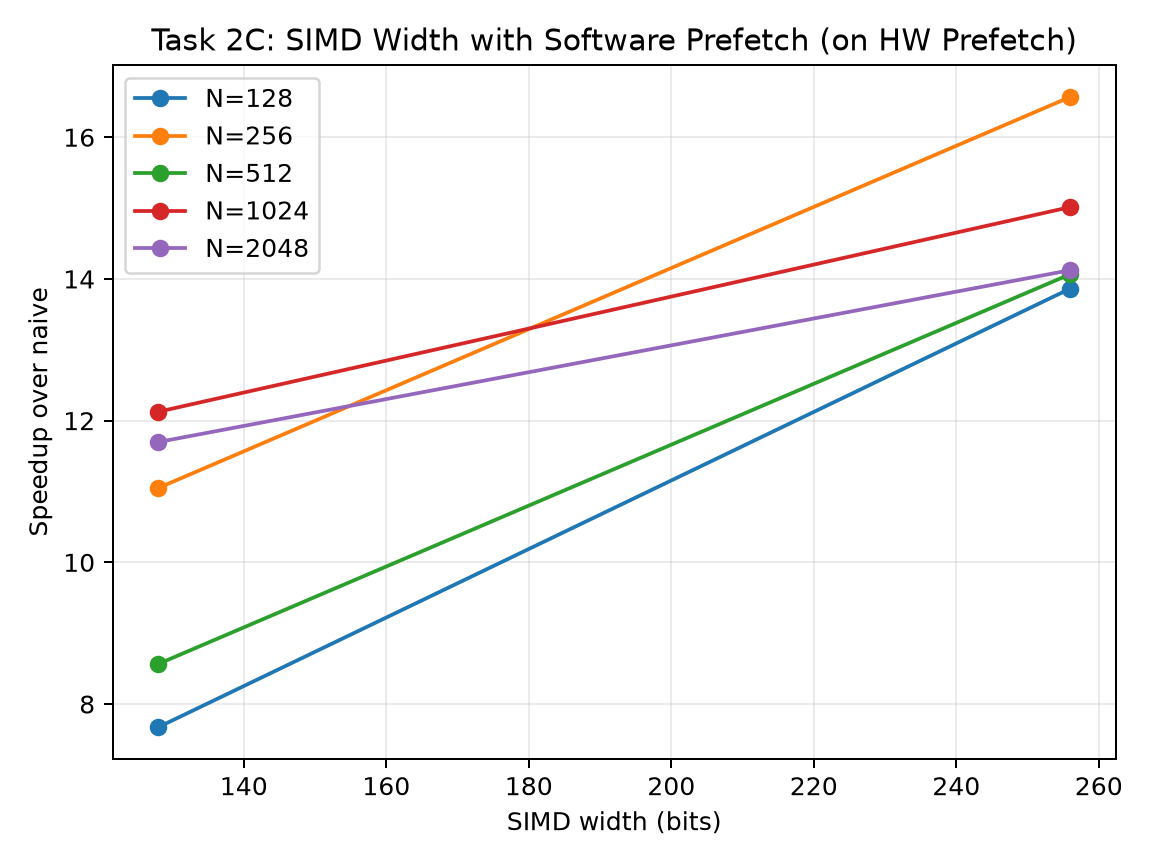
\includegraphics[width=\linewidth]{plots/task2c/task2c_simd_width.png}
        \caption{Speedup vs SIMD Width}
    \end{subfigure}
    \hfill
    \begin{subfigure}{0.48\textwidth}
        \centering
        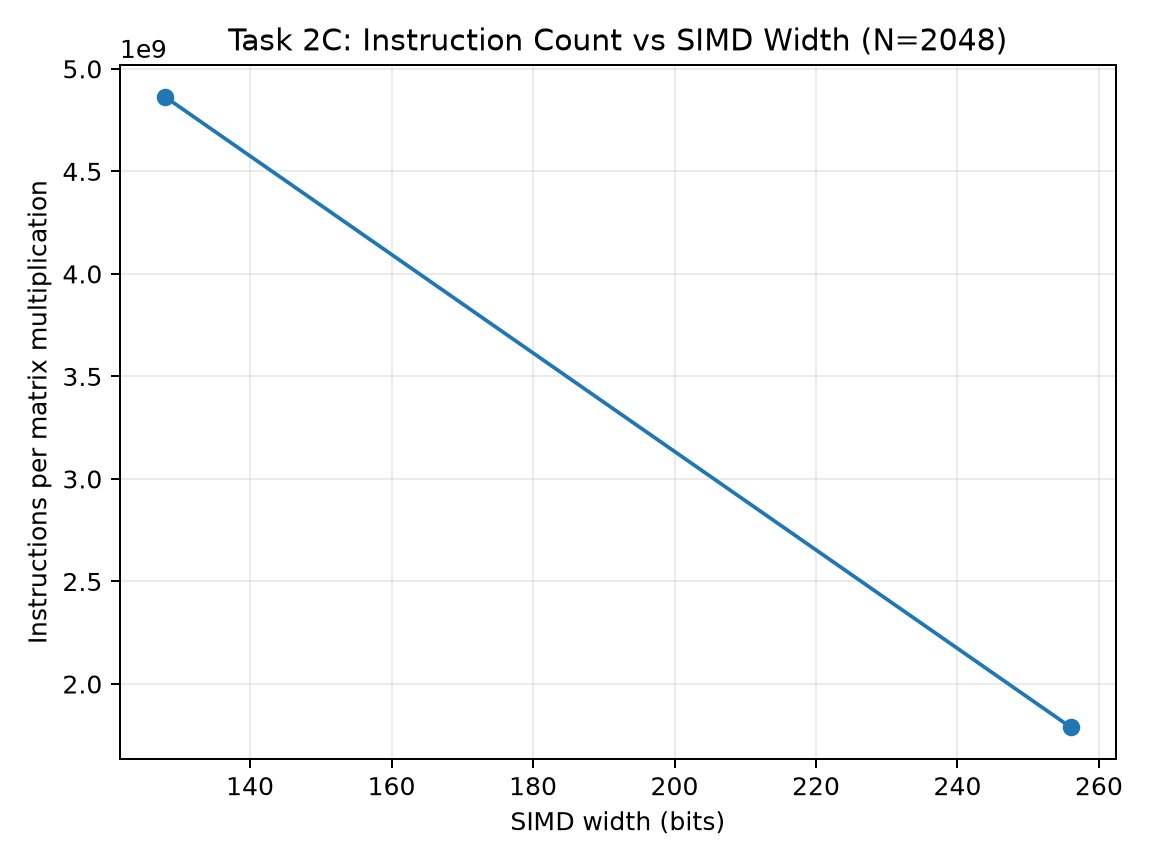
\includegraphics[width=\linewidth]{plots/task2c/task2c_instructions_vs_width.png}
        \caption{Instruction Count vs SIMD Width}
    \end{subfigure}
    \caption{Impact of expanding SIMD width on execution speed and instruction count.}
\end{figure}

\subsubsection{Prefetch Cache Fill Level}
Because of the massive throughput of the 256-bit ALUs, the kernel becomes highly sensitive to memory latency. Consequently, the optimal prefetch cache fill level shifted to \texttt{T0} (L1 cache) across almost all sizes. In Task 2A (scalar), \texttt{T1} (L2 cache) was preferred to avoid L1 thrashing. However, SIMD units require data immediately in the L1 cache; fetching to L2 introduces too much latency for the vector ALUs.

\begin{figure}[H]
\centering
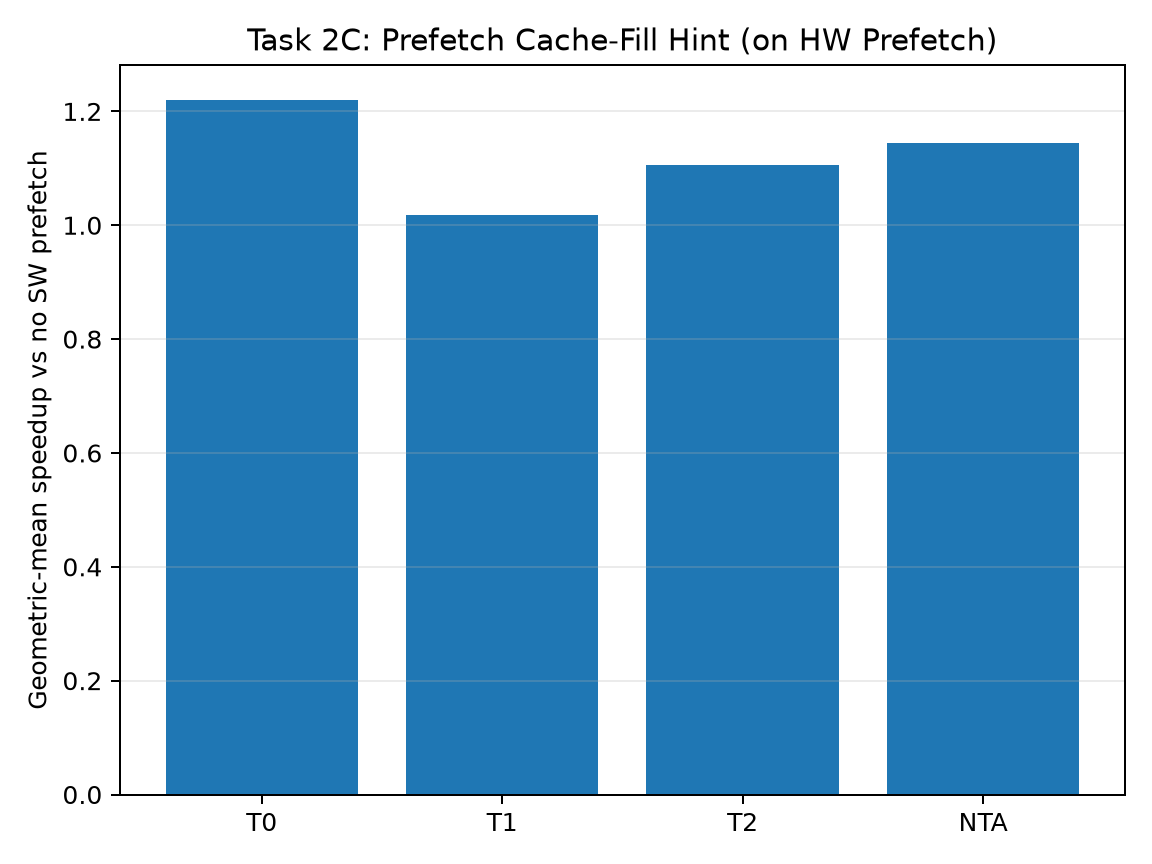
\includegraphics[width=0.6\linewidth]{plots/task2c/task2c_prefetch_level.png}
\caption{Speedup vs Cache Fill Hint (Geometric mean). \texttt{T0} provides the best performance for SIMD workloads.}
\end{figure}

\subsubsection{Prefetch Distance and Cache Metrics}
The geometric mean for the optimal prefetch distance landed at 32 floats, which ensures data arrives just in time without evicting the currently active $32 \times 32$ cache tiles. Requesting data too far ahead (e.g., 512 floats) triggers a noticeable increase in L1D and L2 cache misses, as prefetched data evicts active working sets before they can be fully utilized.

\begin{figure}[H]
\centering
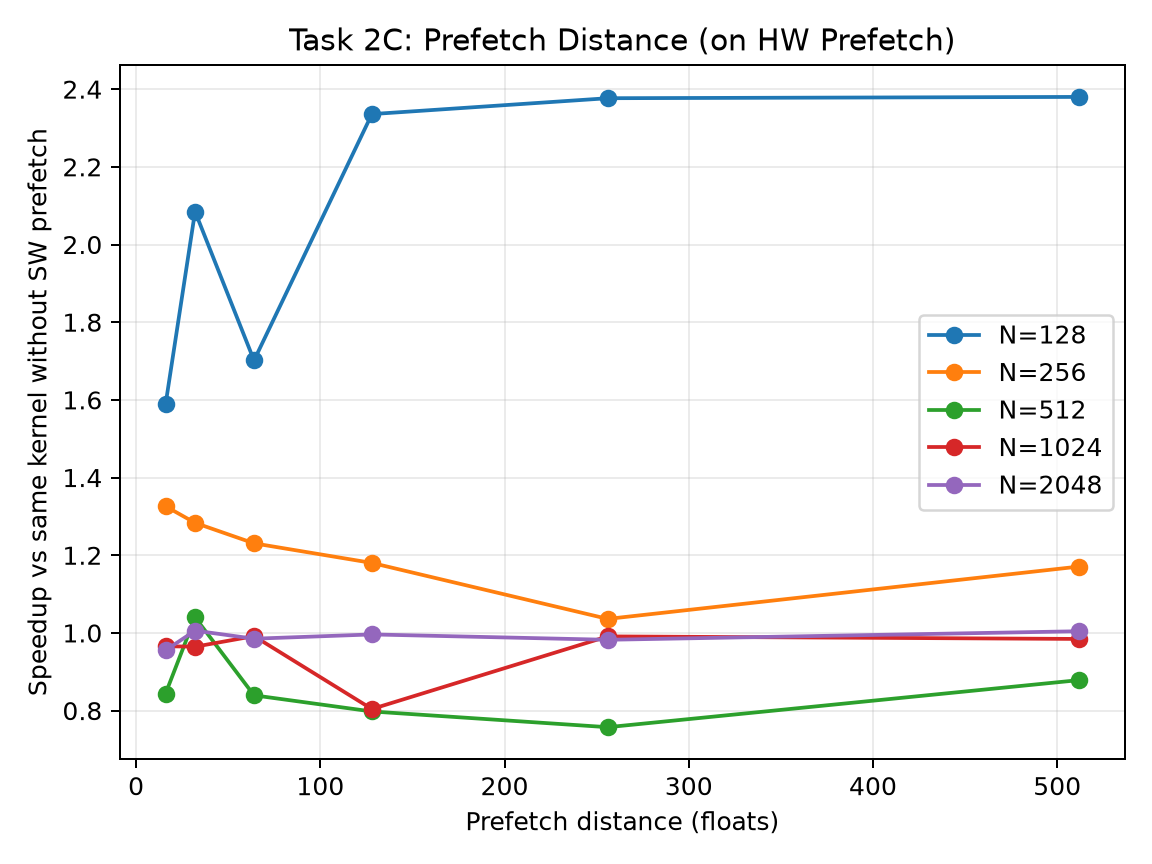
\includegraphics[width=0.65\linewidth]{plots/task2c/task2c_prefetch_distance.png}
\caption{Speedup over baseline (without SW prefetch) across varying prefetch distances.}
\end{figure}

\begin{figure}[H]
    \centering
    \begin{subfigure}{0.48\textwidth}
        \centering
        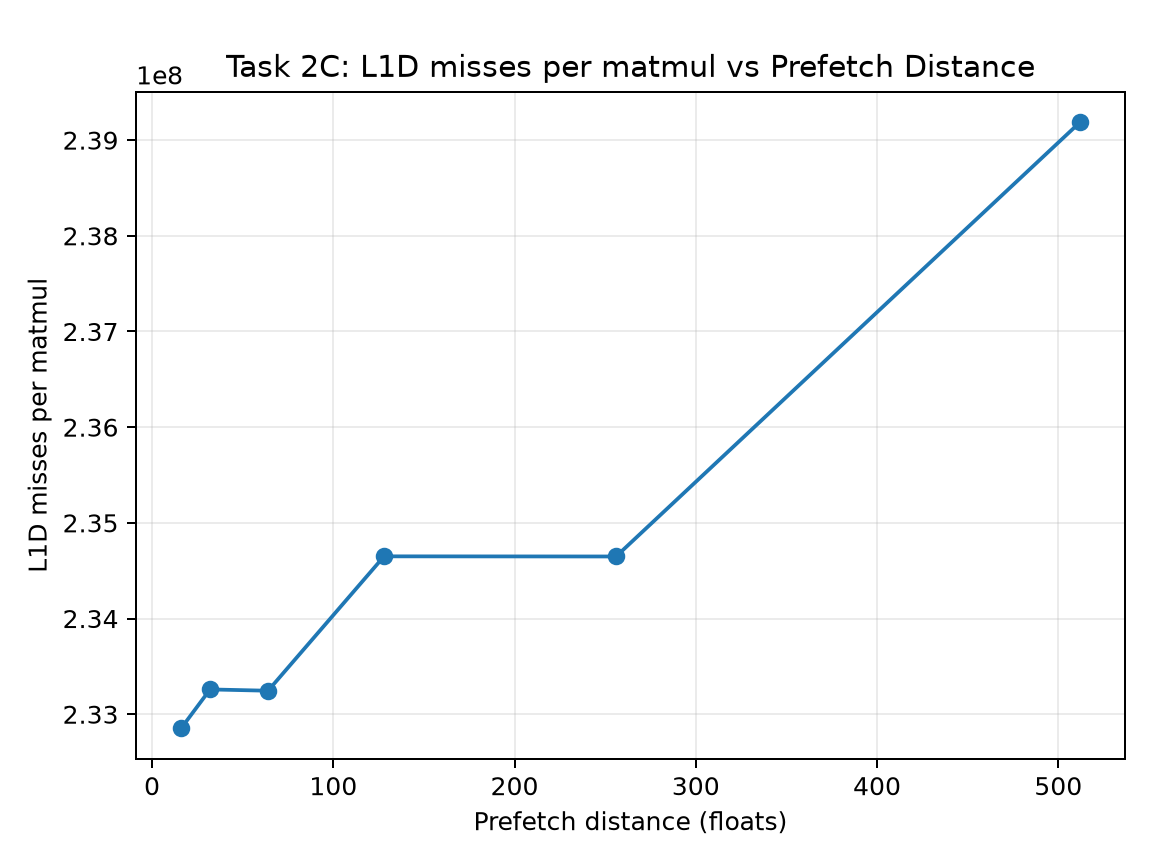
\includegraphics[width=\linewidth]{plots/task2c/task2c_l1d_misses_vs_distance.png}
        \caption{L1D Misses vs Distance}
    \end{subfigure}
    \hfill
    \begin{subfigure}{0.48\textwidth}
        \centering
        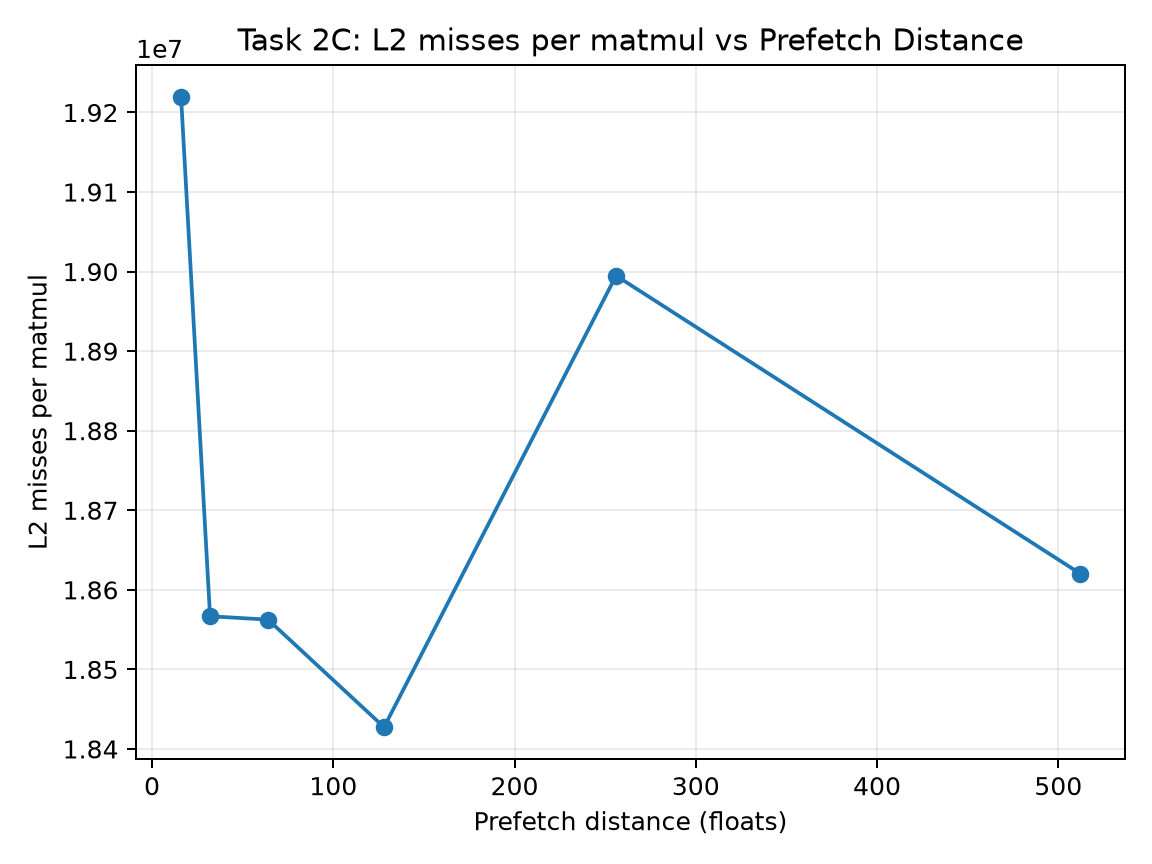
\includegraphics[width=\linewidth]{plots/task2c/task2c_l2_misses_vs_distance.png}
        \caption{L2 Misses vs Distance}
    \end{subfigure}
    \vspace{1em}
    \begin{subfigure}{0.48\textwidth}
        \centering
        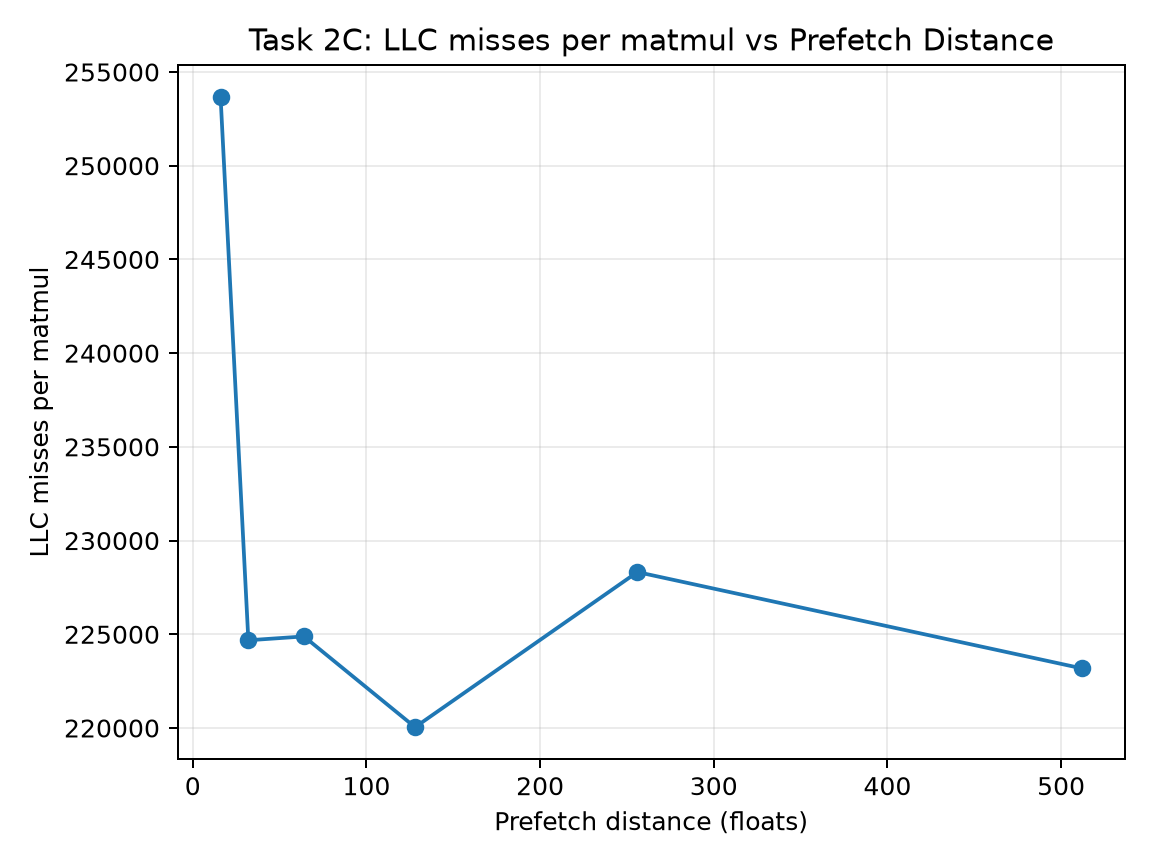
\includegraphics[width=\linewidth]{plots/task2c/task2c_llc_misses_vs_distance.png}
        \caption{LLC Misses vs Distance}
    \end{subfigure}
    \hfill
    \begin{subfigure}{0.48\textwidth}
        \centering
        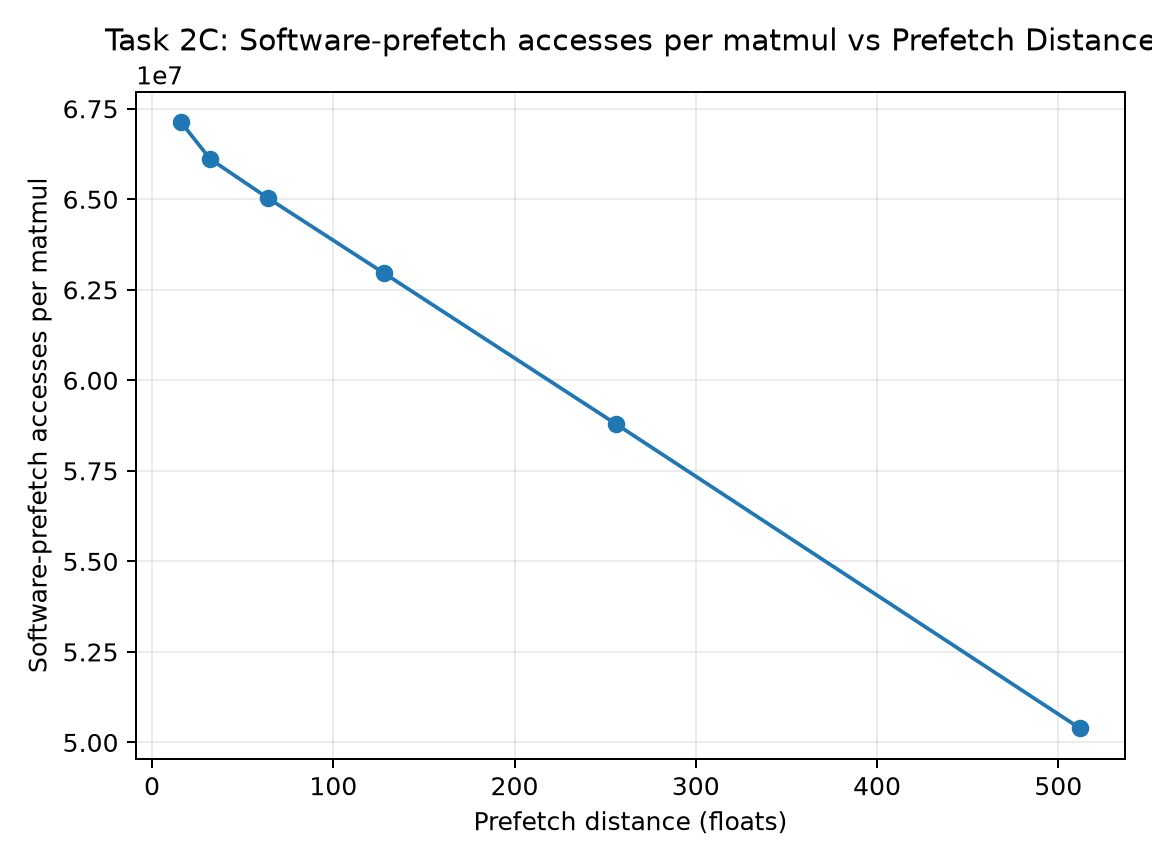
\includegraphics[width=\linewidth]{plots/task2c/task2c_sw_prefetch_access_vs_distance.png}
        \caption{SW Prefetch Accesses vs Distance}
    \end{subfigure}
    \caption{Hardware cache metrics behavior under varying prefetch distances ($N=2048$). Notice the spike in misses at extreme distances.}
\end{figure}

\subsection{Final Performance Comparison}

\begin{figure}[H]
\centering
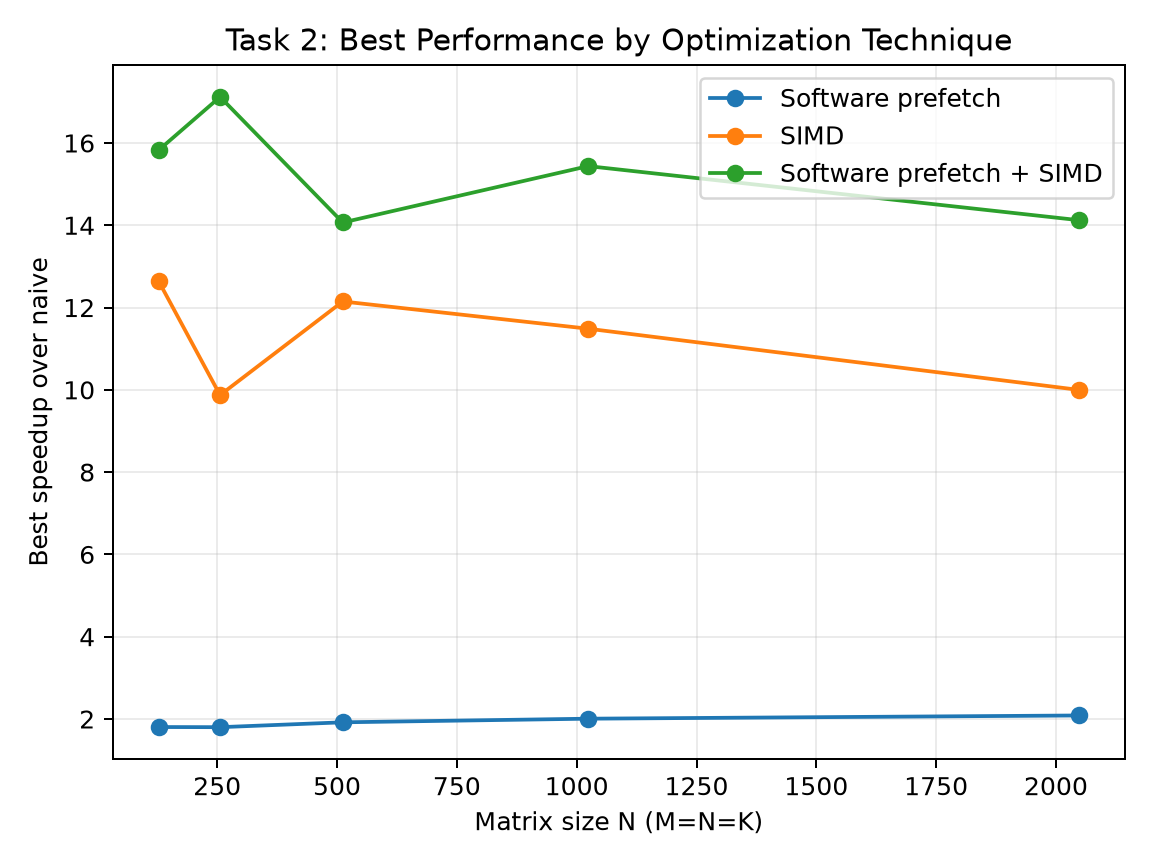
\includegraphics[width=0.8\linewidth]{plots/task2c/task2_final_best_comparison.png}
\caption{Task 2 final performance comparison across optimization techniques.}
\end{figure}

\begin{table}[H]
\centering
\caption{Task 2 final performance summary (Peak observed across sizes)}
\begin{tabular}{lllc}
\toprule
Technique & Peak Speedup & Optimal Hint/Width & Matrix Size at Peak \\
\midrule
Software Prefetching & $\sim 2.08\times$ & Distance 64, Hint T1 & $2048 \times 2048$ \\
SIMD                 & $\sim 12.6\times$ & 256-bit AVX2         & $128 \times 128$ \\
Prefetching + SIMD   & $17.11\times$     & 256-bit, Dist 16, T0 & $256 \times 256$ \\
\bottomrule
\end{tabular}
\end{table}

\subsection{Task 2 Conclusion}
The optimization journey clearly demonstrates that maximum performance requires harmonizing compute and memory architectures. While software prefetching alone provided a modest $\sim 2\times$ speedup by hiding latency, SIMD vectorization delivered a massive $>12\times$ compute boost. 

However, SIMD alone eventually stalls waiting for memory. By combining them—using cache tiling to shrink the working set, SIMD to maximize arithmetic throughput, and \texttt{T0} L1 software prefetching to guarantee data availability—we achieved a highly synergistic peak speedup of $17.11\times$. The combination proves that keeping vector units fed is just as critical as the vectorization itself.

\newpage
% ============================================================
% Results Across Machines
% ============================================================
\appendix
% ============================================================
% Results Across Machines
% ============================================================
\section{Results Across Machines}

To evaluate the portability of our optimizations, we tested the autograder suite on a second machine. The alternative machine achieved a much higher relative speedup ($30.29\times$) than our primary test machine ($22.07\times$), easily clearing the tier to secure the maximum 70 speedup points.

However, absolute execution times reveal our primary machine is substantially faster. It completed the \texttt{optimized} kernel in $21.486$ ms ($\sim100$ GFLOP/s), whereas the alternative machine took $34.174$ ms ($\sim62.8$ GFLOP/s).

\subsection*{Why is the Speedup Higher on a Slower Machine?}

The test harness calculates speedup as a relative metric ($\text{Speedup} = \frac{\text{Execution Time naive}}{\text{Execution Time optimized}}$). The alternative machine's massive $30.29\times$ speedup is primarily driven by its exceptionally poor performance on the scalar \texttt{naive} baseline ($1035$ ms vs. our machine's $474$ ms). 

This ratio discrepancy highlights a few key architectural differences:
\begin{itemize}
    \item \textbf{Hardware Prefetchers:} If our primary machine has a more aggressive hardware prefetcher, it artificially elevates the unoptimized baseline's performance, shrinking the maximum achievable speedup gap.
    \item \textbf{Cache Hierarchy:} The $1024 \times 1024$ default workload intentionally exceeds the L2 cache. A machine with smaller caches or lower bandwidth suffers severe thrashing on naive code, yielding a dramatic relative improvement once cache-blocking is applied.
    \item \textbf{Scalar Execution Efficiency:} Our primary chip likely has superior scalar execution (e.g., higher clocks, better branch prediction), making its baseline much faster. Once SIMD makes both chips heavily compute- and memory-bound, the absolute gap narrows, but the relative ratio skews heavily in favor of the slower machine.
\end{itemize}

\begin{figure}[H]
    \centering
    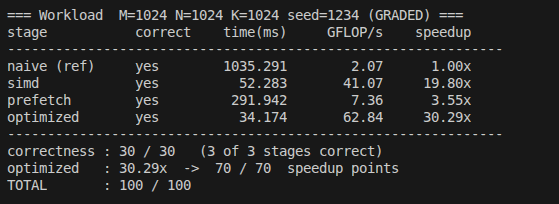
\includegraphics[width=0.85\linewidth]{plots/all_stages_on_different_chip.png} \\
    \vspace{1em}
    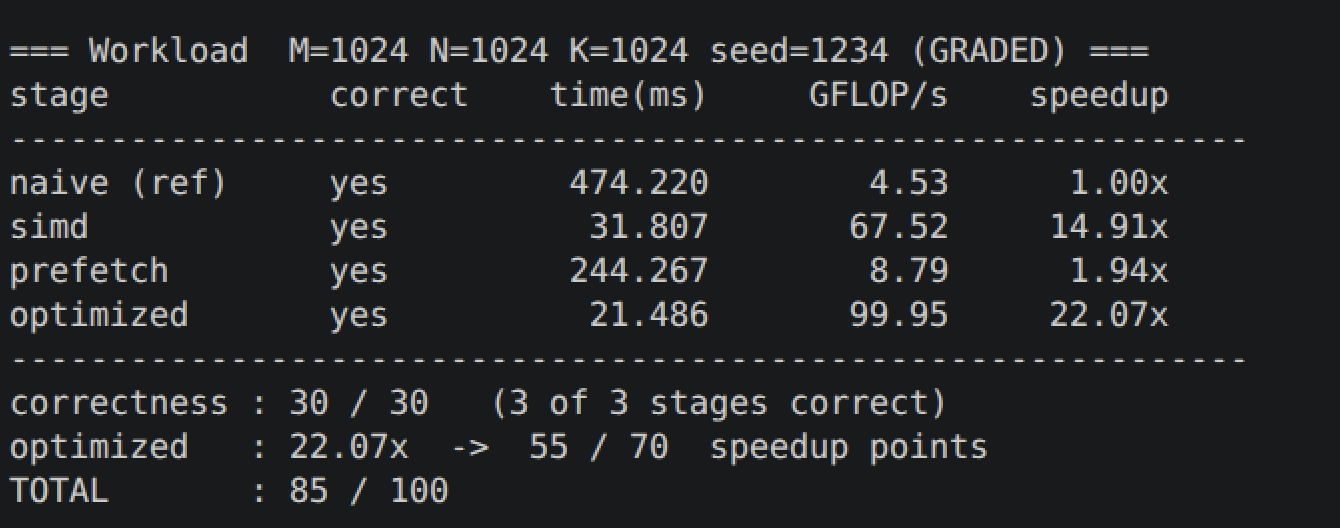
\includegraphics[width=0.85\linewidth]{plots/all_stages_on_our_chip.png}
    \caption{Autograder outputs for $N=1024$. \textbf{Top:} Alternative machine reaching $30.29\times$ speedup. \textbf{Bottom:} Our machine reaching $22.07\times$ speedup, despite having higher absolute throughput.}
\end{figure}
\end{document}